\section{Visão geral do método proposto}
   
   O sistema terá um sensor de captura ótica, que ficará submersos em água, acoplados à uma boia, que terá um conexão sem fio com um celular ou computador.

\begin{figure}[ht]
	\centering
    \caption{\label{fig:bigpic}Visão Geral}
	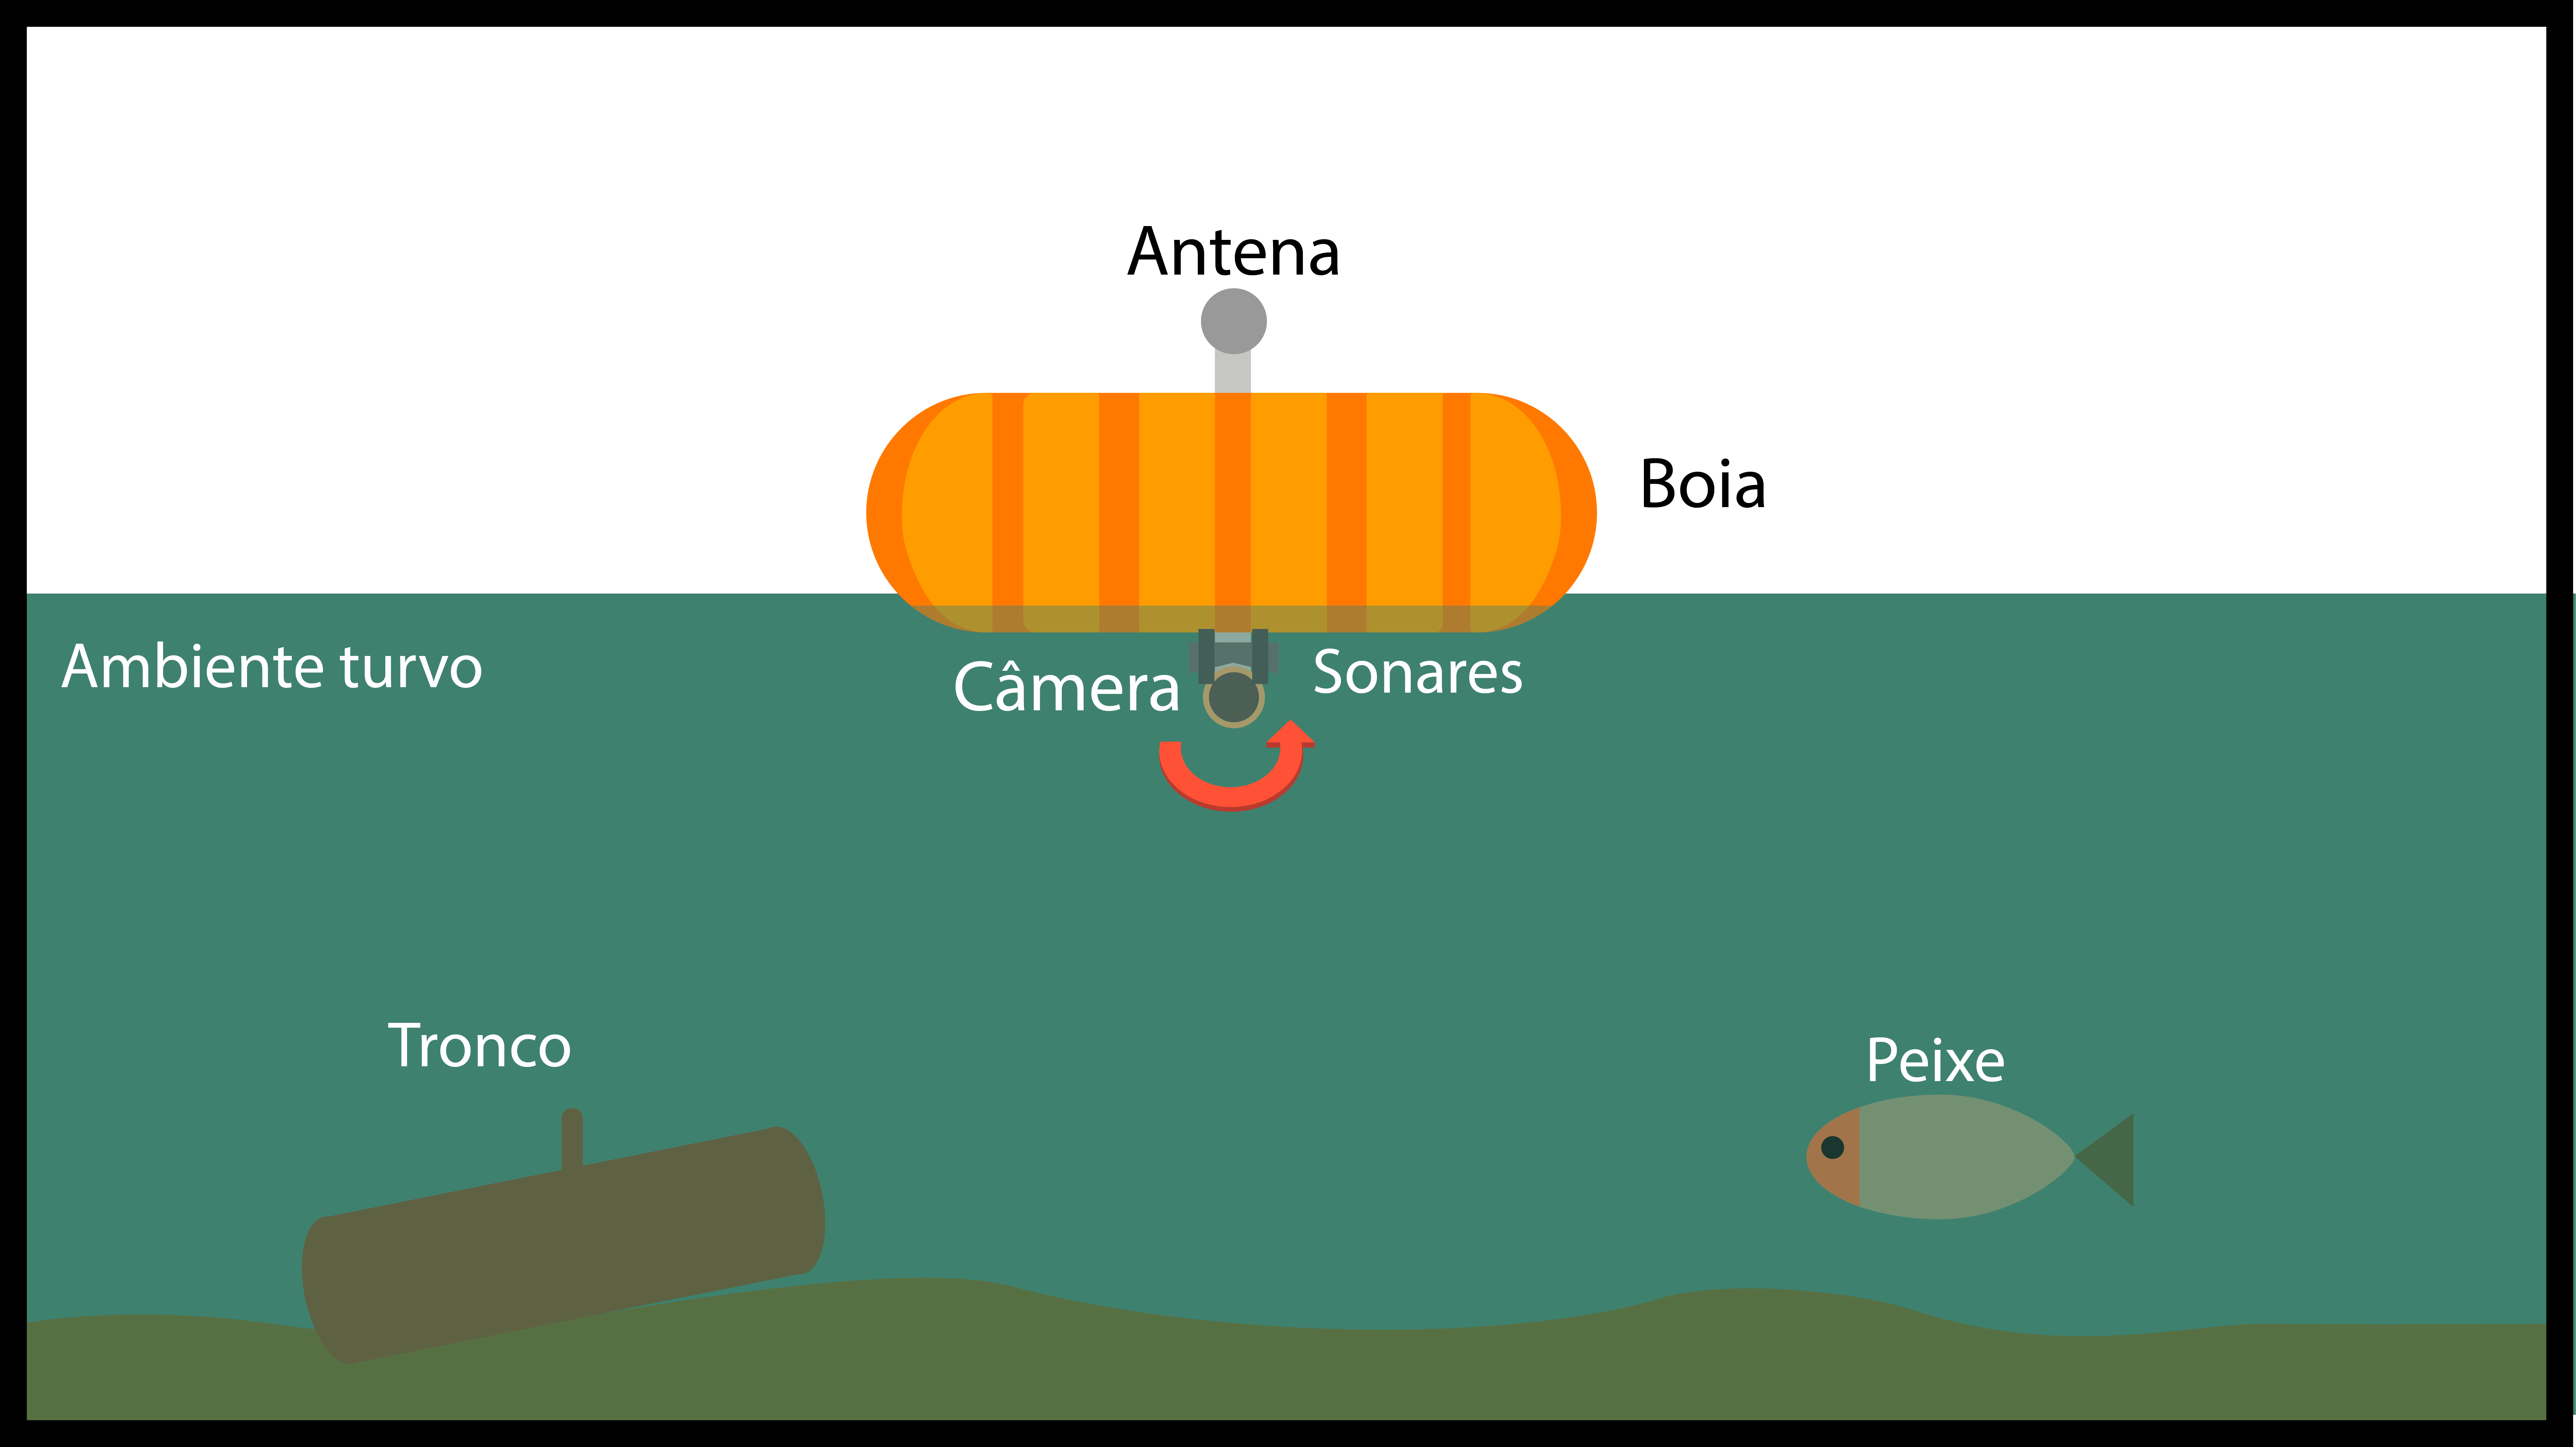
\includegraphics[width = 0.6\textwidth]{resources/Bigpicture}
    \legend{Fonte Própria}
\end{figure}

\section{Identificação de Objetos utilizando openCV}
O método utilizado para nessa primeira fase de identificações consiste nas seguintes etapas. Como mostra a Figura~\ref{fig:fluxfish} 

\begin{figure}[ht]
	\caption{\label{fig:fluxfish}  Fluxo da estrutura do método de identificação de peixes.}
	 \begin{center}
		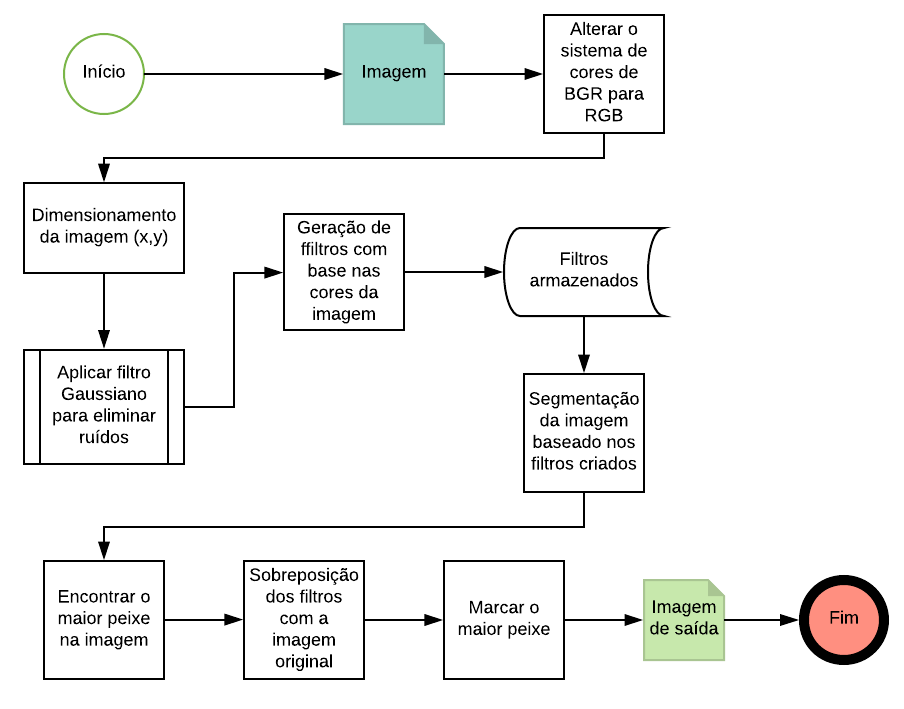
\includegraphics[width = 0.5\textwidth]			{resources/fluxflow}
    \end{center}
    \legend{Fonte Própria}
\end{figure}

\subsection{Pré-processamento}
O pré-processamento da imagem é feito com a correção de cores, alterando seu sistema de cores de RGB para BGR como pode ser visto na figura~\ref{fig:fishp1}. 
\begin{figure}[H]
	\caption{\label{fig:fishp1} Alteração do sistema de cores para RGB}
	\centering
		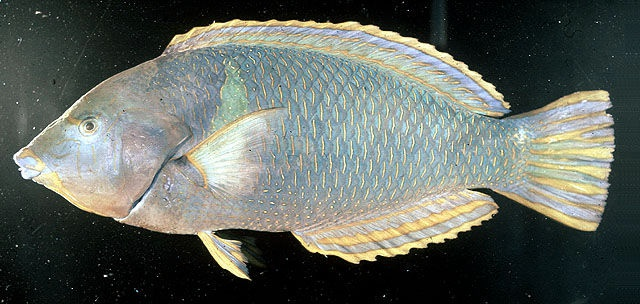
\includegraphics[width = 0.4\textwidth]			{fishes/fish_P1}
    \legend{Fonte Própria}
\end{figure} 
Para remoção de ruídos um filtro Gaussiano com outra modificação no sistema de cores é aplicado, facilitando a identificação de alguns pontos na imagem. o resultado pode ser visto na figura~\ref{fig:fishp2} 
\begin{figure}[H]
	\caption{\label{fig:fishp2} Aplicação de filtro Gaussiano e alteração do sistema de cores para HSV}
	\centering
		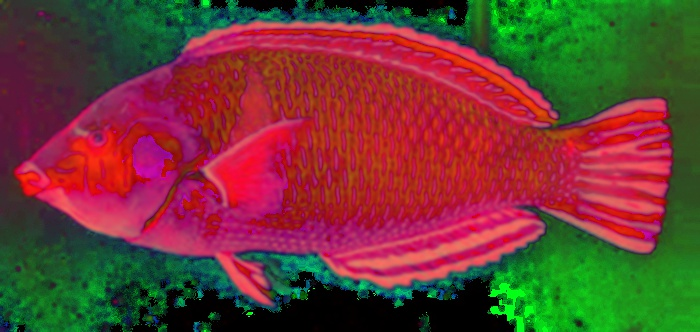
\includegraphics[width = 0.4\textwidth]			{fishes/fish_P2}
    \legend{Fonte Própria}
\end{figure} 

%Em seguida a imagem deve ser livradas de alguns ruídos, assim um filtro gaussiano e conversão do sistema de cores serão aplicados. Resultado na Figura~\ref{fig:fishp2} 


\subsection{Segmentação e identificação de objetos}
A máscara de segmentação é baseada nos níveis de cores encontrados na imagem. Dois filtros são criados com espectros de cores diferentes e em seguida mesclados. . o resultado pode ser visto na figura~\ref{fig:fishp3_mask1}, a figura~\ref{fig:fishp5} mostra a exclusão de segmentos não necessários.
\begin{figure}[H]
	\caption{\label{fig:fishp3_mask1} Extração das máscaras}
	\centering
		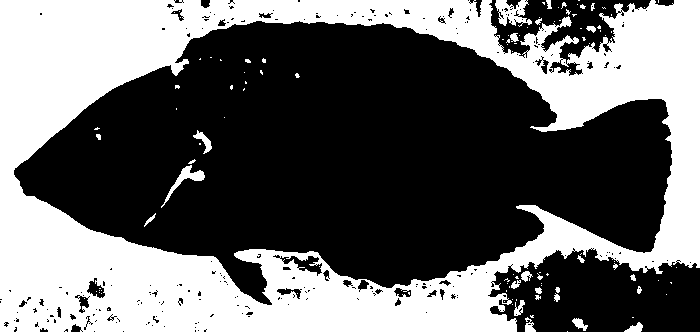
\includegraphics[width = 0.4\textwidth]			{fishes/fish_P3_mask1}
    \legend{Fonte Própria}
\end{figure}
\begin{figure}[ht]
	\caption{\label{fig:fishp5} Exclusão de segmentos}
	\centering
		
\includegraphics[width = 0.4\textwidth]			{fishes/fish_P5_mask_fishes}
    \legend{Fonte Própria}
\end{figure} 

A identificação de objetos na imagem é realizada através da identificação dos maiores pontos encontrados nas máscaras de segmentação, então esses são circulados, gerando a imagem de saída.
\begin{figure}[H]
	\caption{\label{fig:fishp5} Saída}
	 \centering
		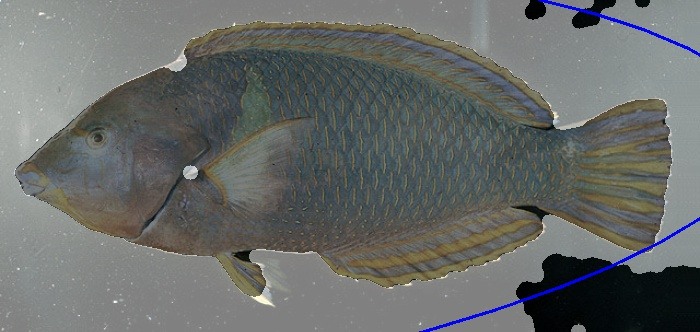
\includegraphics[width = 0.6\textwidth]			{fishes/fish_P7}
    \legend{Fonte Própria}
\end{figure}



